\chapter{7. Project Cost \& Overview}

\section{Cost}

This section covers the cost of the elements needed for the prototypes built in this thesis. It takes into account the materials, machining processes and labor costs.

\subsection{Materials Costs}

The material costs are obtained from the suppliers where the parts were purchased. Overall the project was carried out using already available parts from Changing Places group or MIT Media Lab Machine Shop.

\begin{table*}[hb]
\centering
\begin{tabular}{llll|ll}
\hline
\textbf{Item}                                                & \textbf{Site}     & \textbf{Qty} & \textbf{Price}  & \textbf{Total}  & \textbf{Currency} \\
\hline
Adafruit 9-DOF IMU Fusion Breakout - BNO055 					 & Amazon   & 1   & 32,33  & 32,33  & \$        \\
UNO R3 Board ATmega328P ATMEGA16U2             				     & Amazon   & 1   & 10,86  & 10,86  & \$        \\
18-8 Stainless Steel Male-Female Hex Thread Adapter              & McMaster & 2   & 10,13  & 20,26  & \$        \\
ICAN Carbon Fiber Seat Clamp 31.81mm                             & Amazon   & 1   & 9,99   & 9,99   & \$        \\
Cycling Freewheel Threaded 34 mm                                 & Amazon   & 1   & 3,54   & 3,54   & \$        \\
3 Speed 16-19-22T Thread Freewheel                               & Amazon   & 1   & 14,99  & 14,99  & \$        \\
Threaded Steel 9 Speed 13-32T Freewheel                          & Amazon   & 1   & 15,99  & 15,99  & \$        \\
Super-Swivel Ball Joint Rod Ends                                 & McMaster & 4   & 9,92   & 39,68  & \$        \\
USB-C-HDMI Adapter                                               & Amazon   & 1   & 15,99  & 15,99  & \$        \\
Rod-End Washer Insert                                            & McMaster & 8   & 3,31   & 26,48  & \$        \\
Rotary Motion Position-Measuring Transmitter                     & McMaster & 1   & 307,42 & 307,42 & \$        \\
Polyurethane Wheel for Transmitter Kit                           & McMaster & 1   & 54     & 54     & \$        \\
Signswise 68*118mm Vp-bc73 Bottom Bracket						 & Amazon   & 1   & 14     & 14     & \$        \\
\hline
                                                                 &          &     &        & 565,53 & \$       \\
\hline
\end{tabular}
\\[20pt]
\caption{Material Costs}
\end{table*}

\subsection{Machining Costs}

The two prototypes have been taken into account (the miniPEV and the full scale PEV) throughout all the used processes:

\begin{table*}[h!]
\centering
	\begin{tabular}{l|lllllll|l}
	\hline
	\textbf{Prototype/Process} & \textbf{Waterjet} & \textbf{Laser Cut} & \textbf{3D Printing} & \textbf{Bending} & \textbf{Sand Blaster} & \textbf{Tap} & \textbf{Drilling} &      \\
	\hline
	miniPEV           &          & 12        & 6           & 2       &              &     &          &      \\
	PEV               & 15       &           & 15          &         & 10           & 5   & 6        &      \\
	\hline
	Total Hours       & 15       & 12        & 21          & 2       & 10           & 5   & 6        &      \\
	Cost (\$/h)       & 150      & 40        & 80          & 20      & 30           & 10  & 30       &      \\
	\hline
	Total Cost        & 2250     & 480       & 1680        & 40      & 300          & 50  & 180      & 4980 \\
	\hline
	\end{tabular}
	\\[20pt]
	\caption{Machining Costs}
\end{table*}


\subsection{Labor Costs}

\begin{table}[h]
\centering
	\begin{tabular}{llll}
		\hline
		\textbf{Labor} & \textbf{Unit price (\$/h)} & \textbf{Qty}. & \textbf{Total price (\$)} \\
		\hline
		Research Assistant     & 12                & 1400 & 16800            \\
		Principal Investigator & 85                & 10   & 850              \\
		\hline
		Total                  &                   &      & 17650           \\
		\hline
	\end{tabular}
\caption{Labor Costs}
\\[20pt]
\end{table}

\newline
\\
The labor costs are estimated from the annual salaries of the involved members and the machining costs are estimated from Ulrich \& Eppinger's Product Design and Development \cite{ulrich2004product}.

\subsection{Total Cost}

\begin{table}[h]
\centering
\begin{tabular}{cc}
		\hline
		\textbf{Part}      & \textbf{Total price (\$)} \\
		\hline
		Materials & 565.53           \\
		Machining & 4980             \\
		Labor     & 17650            \\
		\hline
		\textbf{Total}     & \textbf{23195.53}     \\
		\hline   
	\end{tabular}
\caption{Total Cost}
\\[30pt]
\end{table}

\section{Project Timeline}

A Gantt chart with the main tasks of the project has been included.

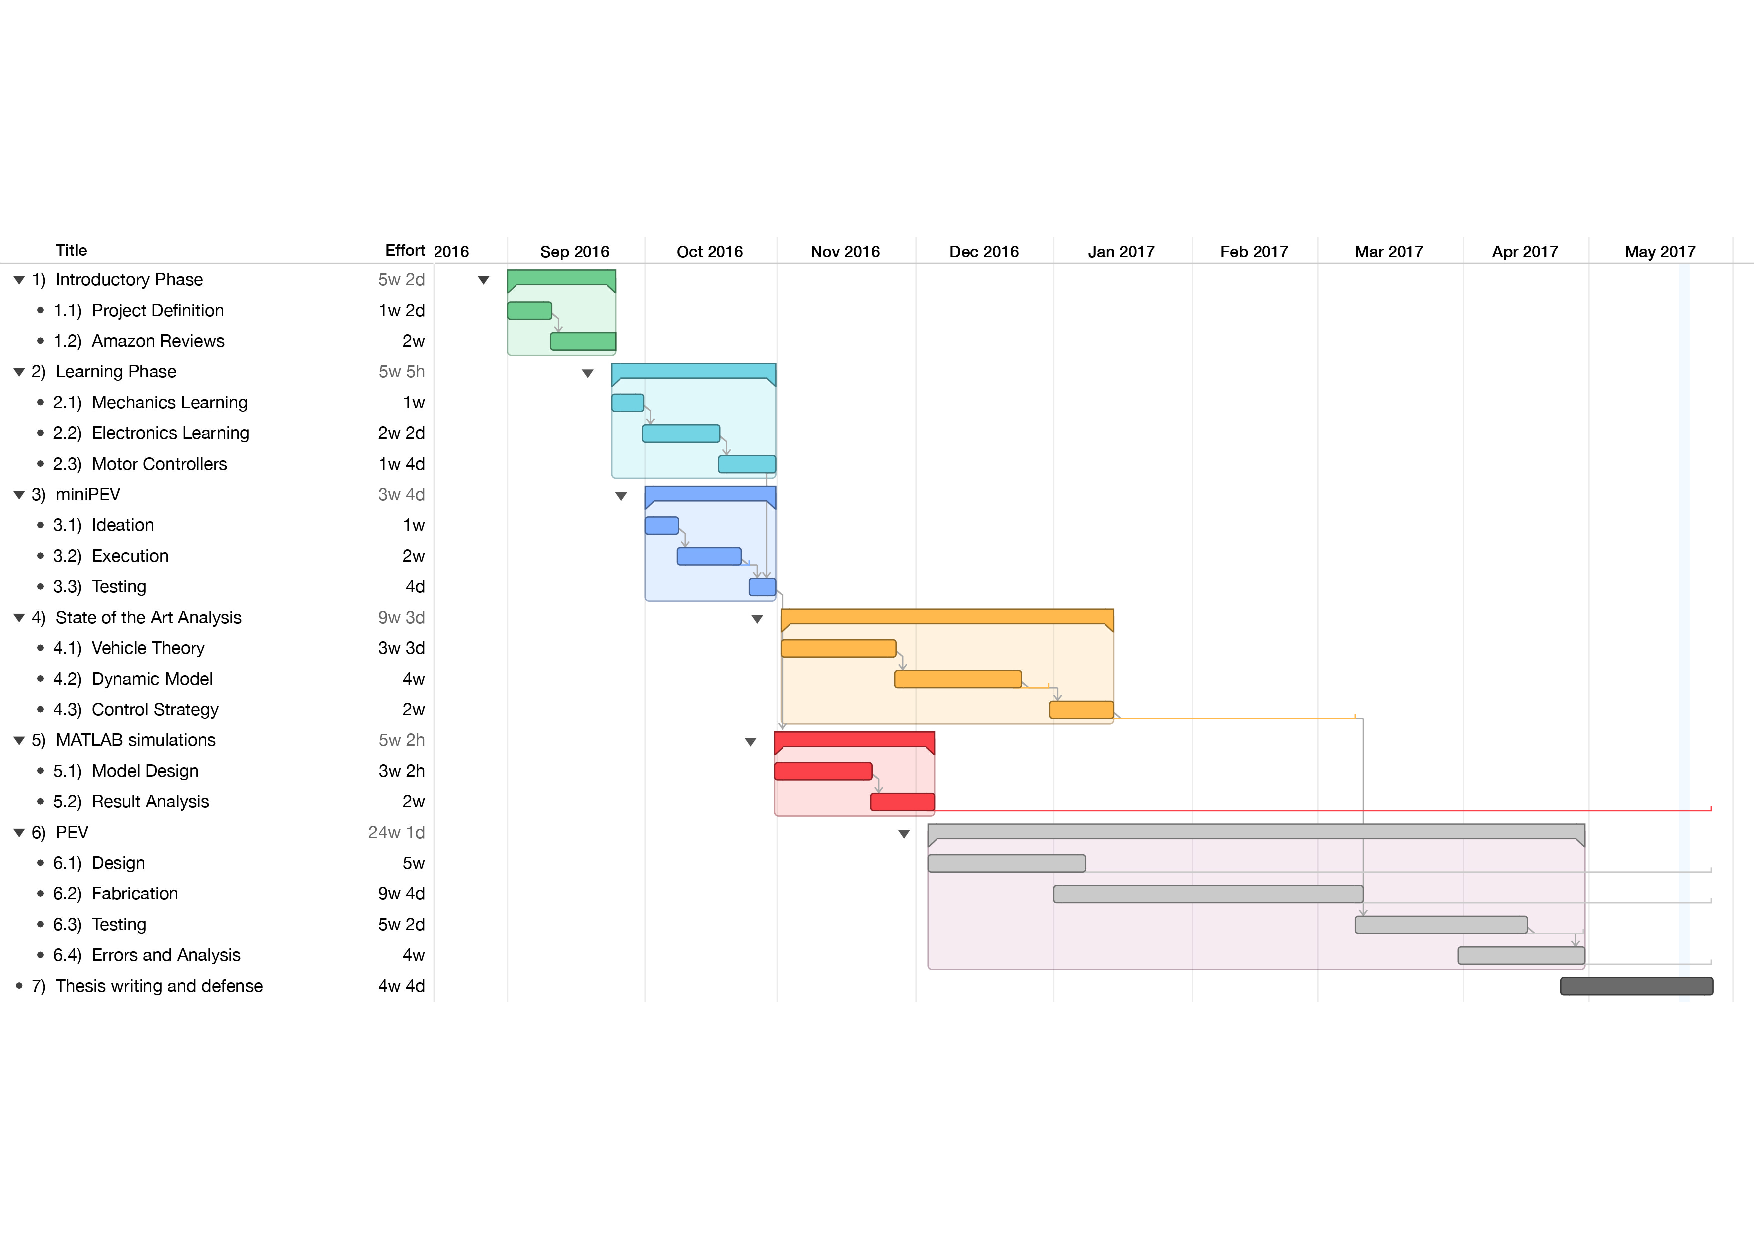
\includepdf[pages=-	,fitpaper,scale=1,pagecommand={\label{timeline}}]{figs/07/Timeline2.pdf}
